\section{Method}\label{method}

In this section we describe our method, that follows the one adopted in \cite{NIPS2018_8025}.

\subsection{Training Protocol}\label{Alg}
In IRL has to be defined three basic components: the \textit{policy} that specify how the agent moves in the environment; an \textit{annotator} which gives preferences to clips; and a \textit{reward model} that estimates a reward function from the provided preferences. 

The training phase of our system follows the protocol described in the Algorithm\ \ref{alg:train_proto}, where the policy and the reward model are jointly trained.

\begin{algorithm}
\caption{Training Protocol}
\label{alg:train_proto}
\SetAlgoLined
\begin{algorithmic}[1]
\STATE Run the policy in the environment and store "initial trajectories".
\STATE The annotator annotated all the "initial clips" and create the annotation buffer.
\STATE Pretrain the reward model from the annotation buffer.
\FOR{\textit{M} epochs} 
\STATE Train the policy in the environment for \textit{N} episodes with rewards from the reward model.
\STATE Sample pairs of clips from the resulting trajectories.
\STATE The annotator labels the selected pairs and puts them in the annotation buffer.
\STATE Train the reward model for \textit{K} batches from the annotation buffer.
\ENDFOR 
\end{algorithmic}
\end{algorithm}
 
We achieve our best configuration with $N=150$ policy episodes and $K=1500$ reward model batches. %at the $21^{st}$ iteration

The number of sampled clips decreases as the number of epochs increases. In particular, the annotator labels the $100\%$ of clips at first iteration and, every 5 iterations, that percentile decreases by $20\%$. 
\subsection{Policy}
During the training of the policy, the agent interacts with the environment over a number of time steps (that we set to a maximum of T = 150). In time step $t$ the agent receives an observation $o_t$ from the environment and it performs an action $a_t$. This action is chosen with a sampling of a Categorical distribution where the logits are the output values of the policy model giving $o_t$. A trajectory is the set of couples ${(o_1, a_1), (o_2, a_2), \ldots, (o_T, a_T)}$. If the agent reaches the goal state in a step $\textit{t}<T$, we terminate this episode before the agent has done all the steps.

Typically, in Reinforcement Learning, the agent receives a reward $r_t$ at each step from the environment, but in Inverse Reinforcement Learning the reward model plays this role. The advantage consists of providing the agent non-zero rewards before reaching the environment goal. The MiniGrid reward function give non-zero reward only in the environment goal.
Furthermore, in complex environment, the agent spends a lot of steps to reach the goal and to learn the environment rules because of sparse rewards. The reward model, instead, provides dense rewards to the agent from the begging of its episodes. 

Our policy model is inspired to the one presented in \cite{karpathy}, this is a fully connected layer with 64 hidden units and ReLU activation followed by another fully connected layer with 7 output units (that are clamped from -1000, 1000). The input to the model are the agent observations at each agent step. 

For our experiments we adopt Adam optimizer with $0.0001$ of learning rate and we regularize that with $0.01$ of weight decay. 

\subsection{Annotator}
The aim of the annotator is to give preference feedback about segments of agent trajectories, called \textit{clip}. A clip consists of 5 consecutive agent trajectory's elements $\{(o_i, a_i)_{i=t}^{t+4}\}$. Since the trajectory can have variable dimension (e.g. when the agent reaches the environment goal), we create a clip generator able to create clips of a fixed length from a trajectory. If the agent reaches the environment goal during this trajectory at time stamp $t$, with $t \mod T \not= 0$, our generator creates the last clip with the goal state replicated several times in order to create another clip with the same length.

After the clips generation, the annotator has to label pairs of sampled clips. In our experiments the sampling is uniform and without bootstrapping. The only possible values for a single preference provided by the annotator are $(1,0)$, $(0,1)$, $(0.5,0.5)$ or $(0,0)$. In the first two chances, the annotator prefers one clip with respect to the other; when the preference is $(0.5,0.5)$ we got two \textit{indifferent labels}; the last possibility refers to a discarded couple of clips, that will be deleted from the training process. The indifferent labels match to two clips where it's impossible to give a preference feedback, and those annotations produced an unusual result: the more their number is, the more the reward model loss will be. For more details about that, please refer to Section \ref{05}.

The annotator has to force the agent to take a specific route in the environment, and to reach this goal we have to annotate only clips with agent steps in this direction. Even if, in a clip, the agent takes only one step in one position that is not in this direction, we reject the clip. 

In this paper we analyze two different types of preference feedback: those provided by a human annotator, and those given by an artificial one, that we call Oracle. Human preferences are collected by our IRL Tool, described in Section \ref{04}, where we support the user during the annotation process with a GUI. Instead, the Oracle gives preferences based on handcrafted rules.

The result of the annotation process is the annotation buffer, that is a set of triples $\{(\sigma^1_i, \sigma^2_i, \mu_i)\}$, where $\sigma^1, \sigma^2$ are two clips and $\mu$ represents the provided preference. We reset the annotation buffer each iteration of the training protocol (see Algorithm\ \ref{alg:train_proto}) and we never put the discarded pairs of clips ($\mu=(0,0)$) in the annotation buffer.


\subsection{Reward Model}
The reward model $\hat{r}$ is a preference predictor, its target is to emulate how the annotator labels each pair of clips. To achieve this goal, it is assumed that the annotator's probability of preferring a segment $\sigma^i$ depends exponentially on the value of the reward summed over the length of the segment\ \cite{NIPS2018_8025}:
\begin{equation}
    \hat{P}[\sigma^1 \succ \sigma^2] = \frac{exp(\sum_{o \in \sigma^1} \hat{r}(o))}{exp(\sum_{o \in \sigma^1} \hat{r}(o) + \sum_{o \in \sigma^2} \hat{r}(o))}
\end{equation}

%%%%%%%%%%%%%%%%%%%%%%%%%%%%%%%%%%%%%%%%%%%%%%%%%%%%%%%%%%%%%%%%%%%%%%%%%%%%%%%%%%%%%%%%%%%%%%
\begin{figure*}[t]
    \qquad
	\subfloat{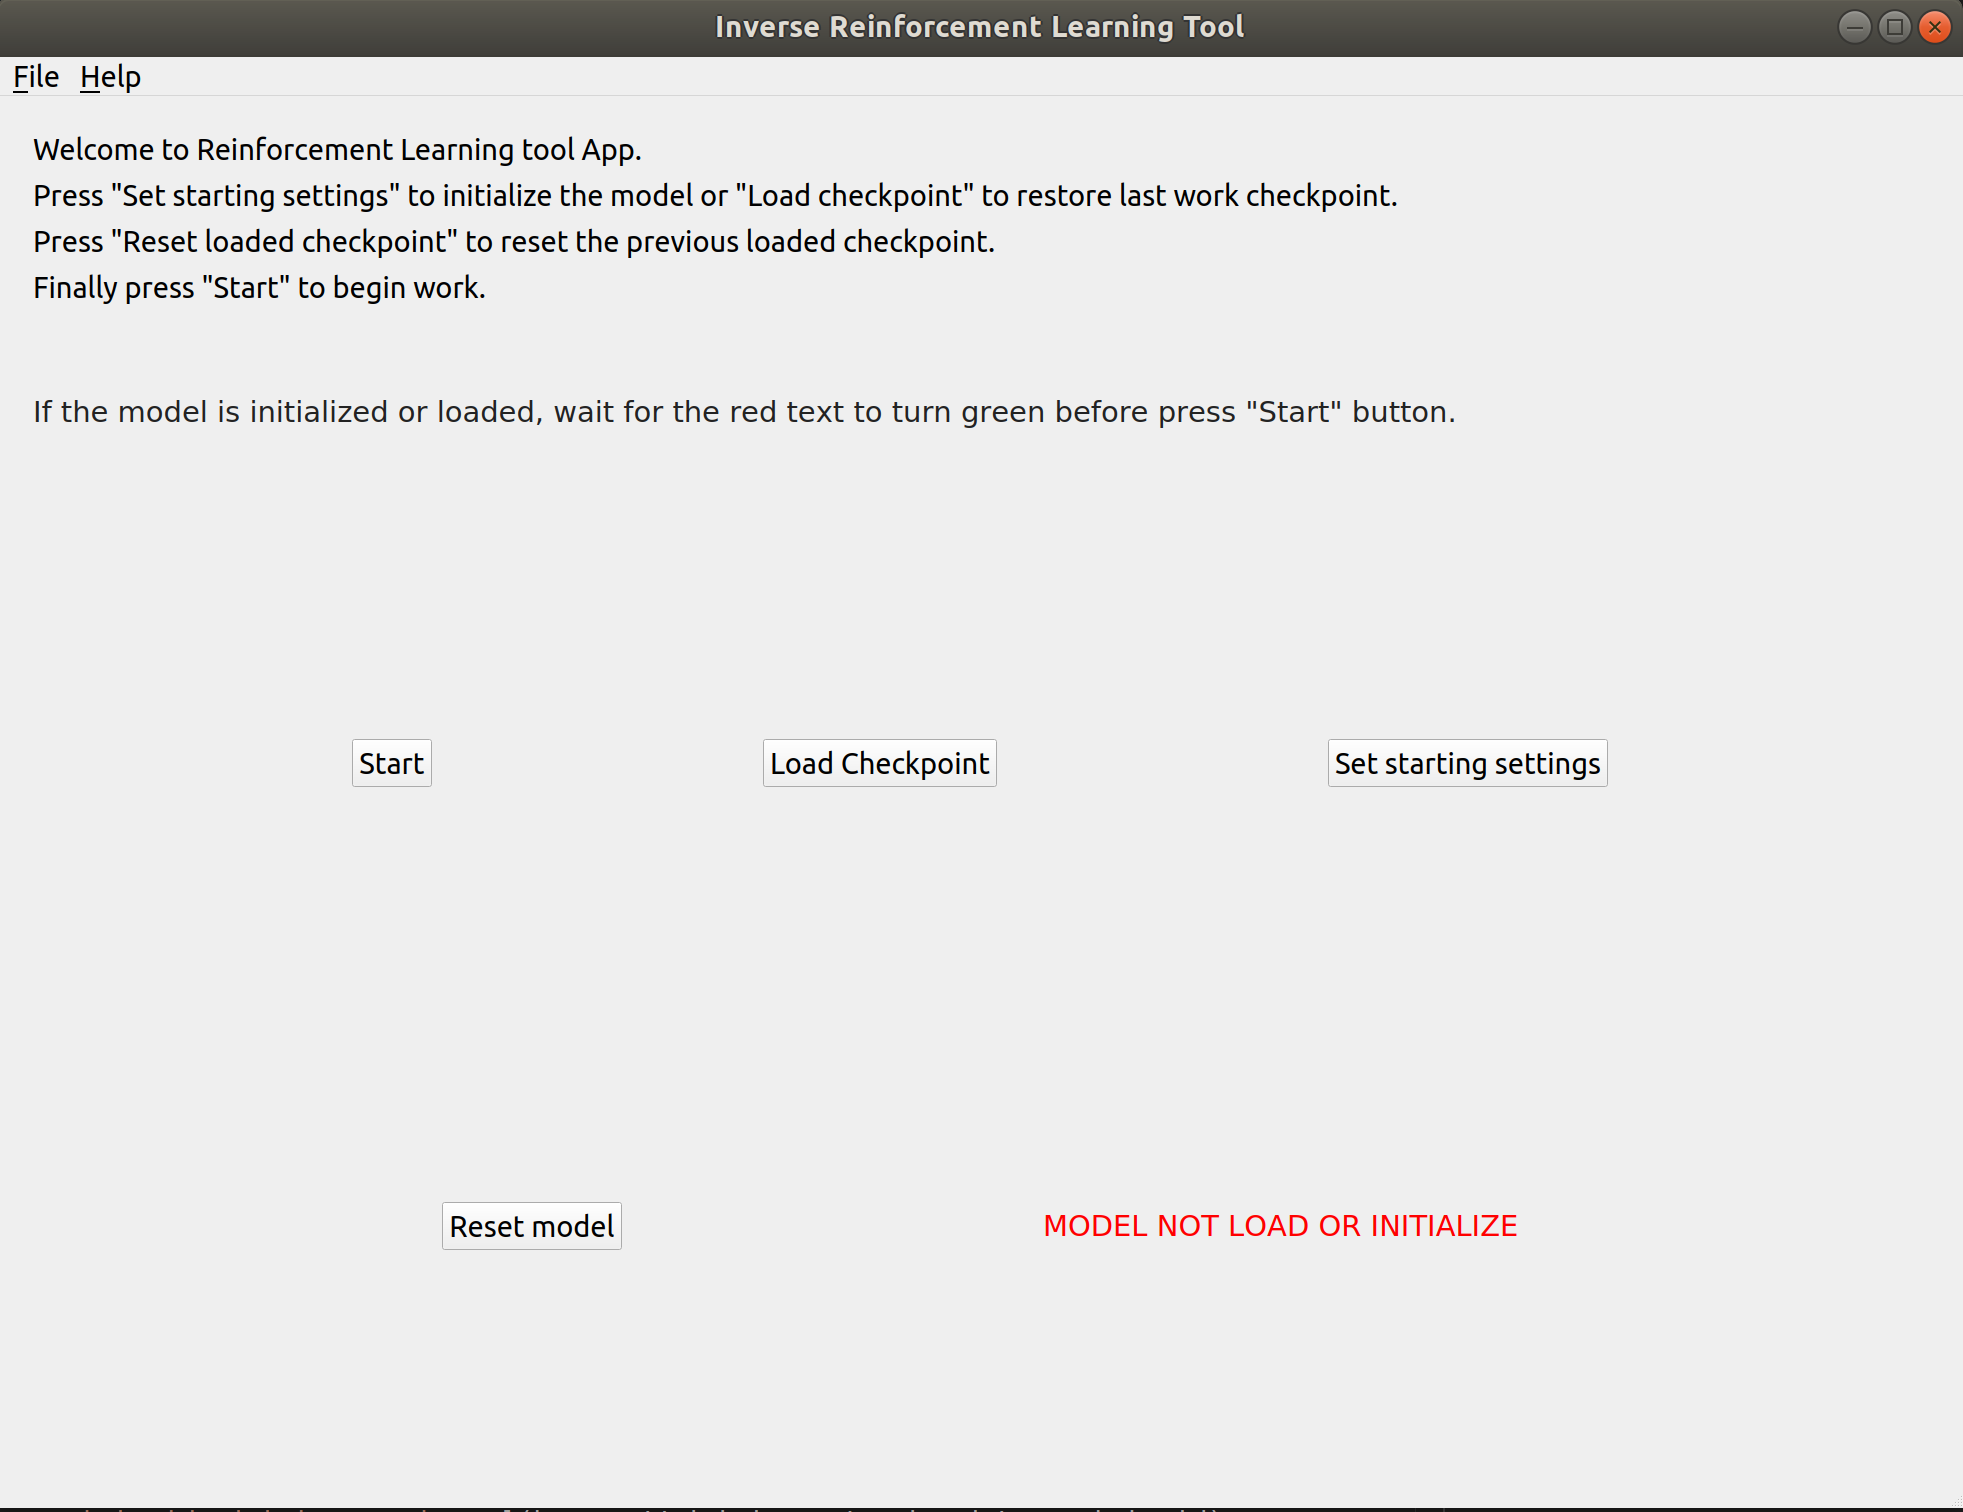
\includegraphics[width=0.30\linewidth]{data/main_view.png} }%
	\subfloat{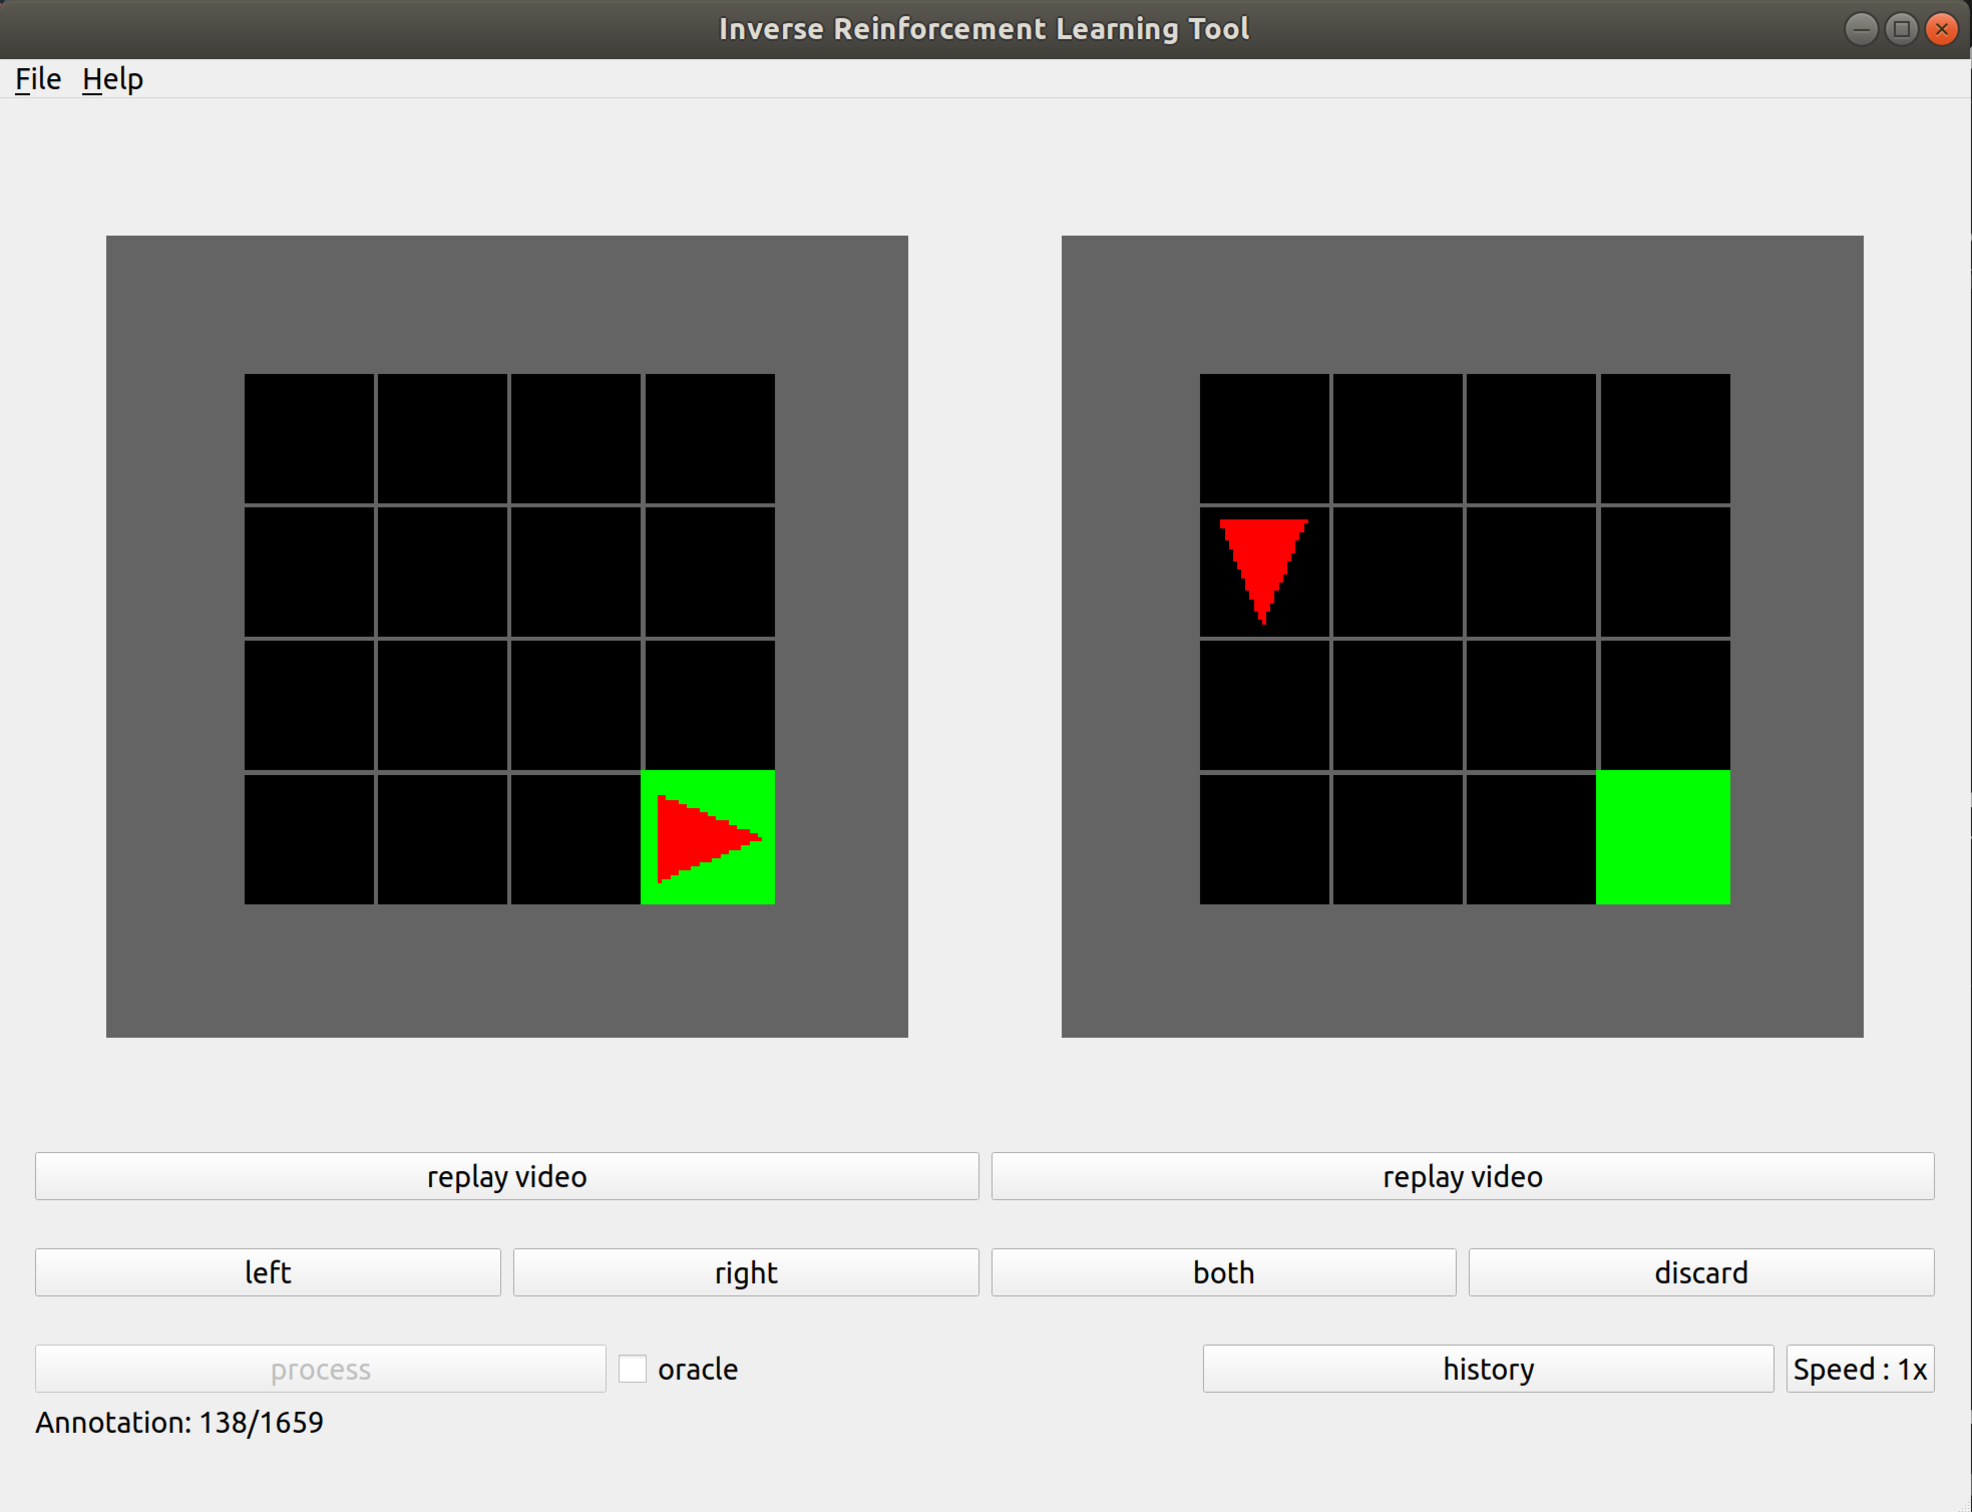
\includegraphics[width=0.30\linewidth]{data/alg_view.png} }%
	\subfloat{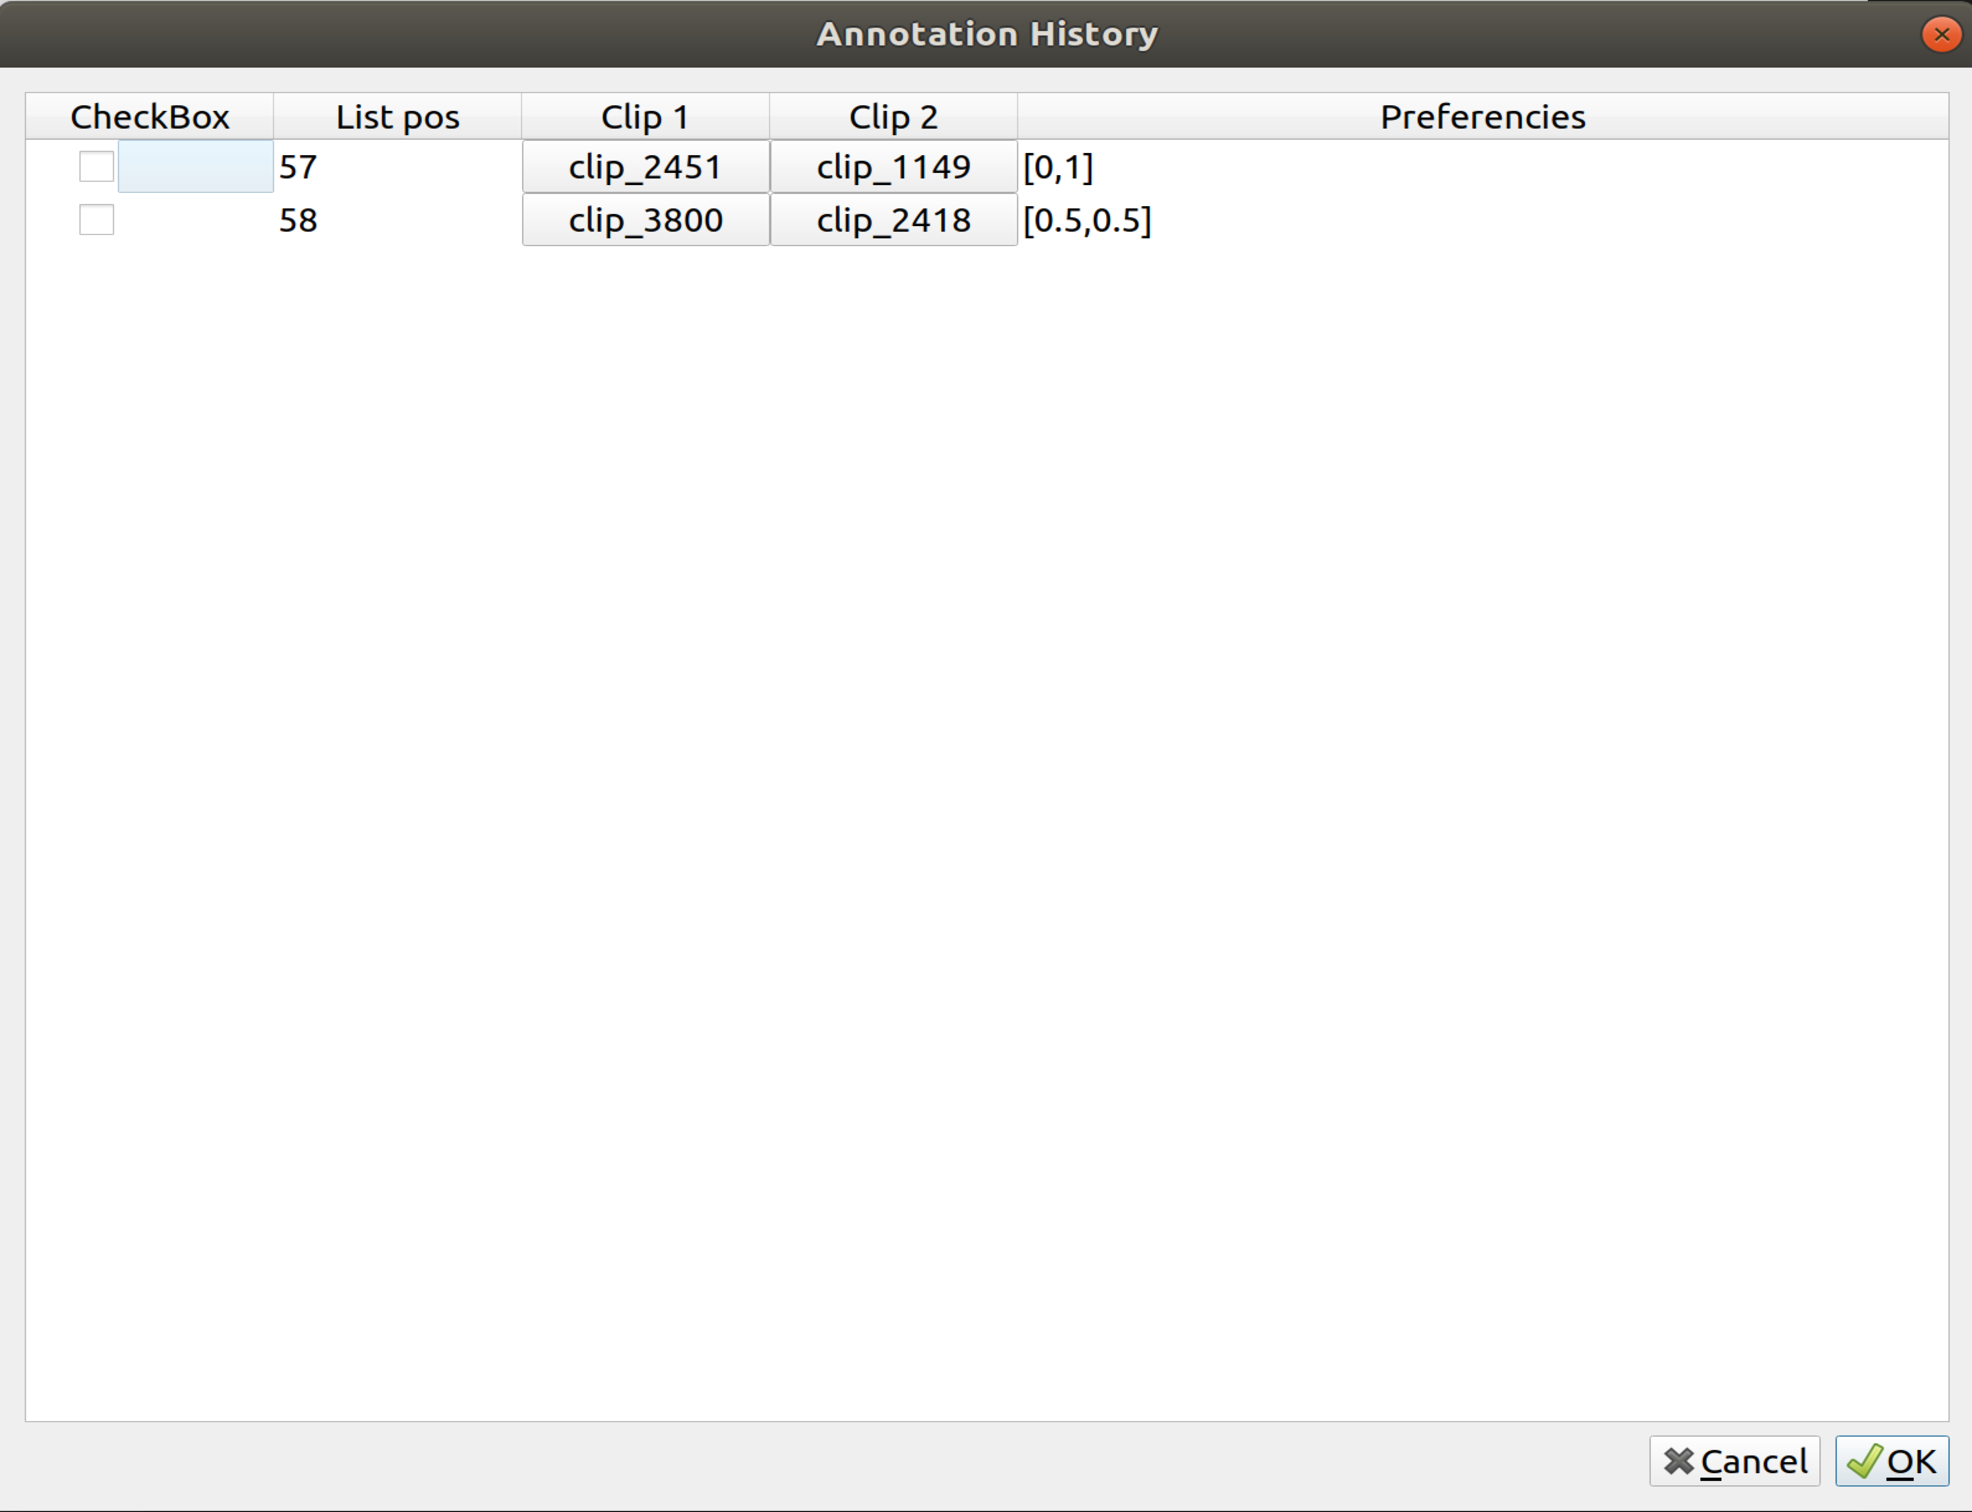
\includegraphics[width=0.30\linewidth]{data/history_window.png} }%
	\caption{Different application views. The first is the Main Window, that is the configuration panel. The second represent the implementation of the training protocol, that supports the annotation process. The last window is the History Panel.}%
	\label{fig:Application}%
\end{figure*}
%%%%%%%%%%%%%%%%%%%%%%%%%%%%%%%%%%%%%%%%%%%%%%%%%%%%%%%%%%%%%%%%%%%%%%%%%%%%%%%%%%%%%%%%%%%%%%%

So the reward model $\hat{r}$ is trained to minimize the cross-entropy loss between these predictions and the actual judgment labels:
\begin{equation}\label{eq:rewardloss}
    loss(\hat{r}) = - \sum_{(\sigma^1,\sigma^2,\mu)\in A} \mu(1)log(\hat{P}_{1,2}) + \mu(2)log(\hat{P}_{2,1})
\end{equation}
where $\hat{P}_{i,j} = \hat{P}[\sigma^i \succ \sigma^j]$. This follows \cite{10.1093/biomet/39.3-4.324}, where is described how to estimate score function from pairwise preferences. Since the reward model is trained on an annotation buffer relatively small (100-200 triples), we use L2 regularization during the optimization process (with $\lambda = 0.01$). Furthermore, we standardize the output of the reward model over the last 300 predicted rewards to have 0 mean and 0.5 standard deviation (those are empirical values, see Section \ref{05} for more details).

Our reward model is a MLP net with two fully connected layers: the first with 64 hidden units and ReLU activation and the second with one output unit without any activation function. For our experiments we adopt Adam optimizer with $0.0003$ of learning rate.
The input to the model are two clips $\sigma^1$ and $\sigma^2$ both composed by 5 consecutive agent observations. For each clip we compute the output of the model, that is a list of 5 rewards, one for each agent state present in the processed clip. 

During the training phase, the reward model performs over the annotation buffer K batches each consisting of 16 sampled triples with bootstrapping, because of the small dimensions of the training set. 

